\chapter{DESAIN DAN IMPLEMENTASI SISTEM}
\label{sec:chap3}

\section{Deskripsi Sistem}

Bab ini menjelaskan perancangan dan implementasi sistem robot inspeksi berbasis agen \textit{Large Language Model} (LLM) yang dibangun di atas platform Jueying Lite3. Sistem ini dirancang agar operator dapat mengendalikan robot melalui instruksi bahasa alami, di mana agen AI akan secara otonom merencanakan dan mengeksekusi misi inspeksi secara bertahap dengan verifikasi di setiap langkahnya.

\subsection{Gambaran Umum Sistem}
Secara garis besar, sistem yang diusulkan dirancang untuk menjembatani kesenjangan komunikasi antara operator manusia dan robot \textit{quadruped} melalui antarmuka bahasa alami. Berbeda dengan metode teleoperasi konvensional yang mengandalkan kendali manual penuh, sistem ini menempatkan \textit{Large Language Model} (LLM) sebagai unit pemroses logika pusat yang mengorkestrasi alur informasi dari instruksi pengguna hingga eksekusi fisik robot. Skema interaksi ini mengubah paradigma pengendalian robot dari yang sebelumnya bersifat teknis dan kaku menjadi lebih intuitif dan semantik.

\begin{figure}[H]
    \centering
    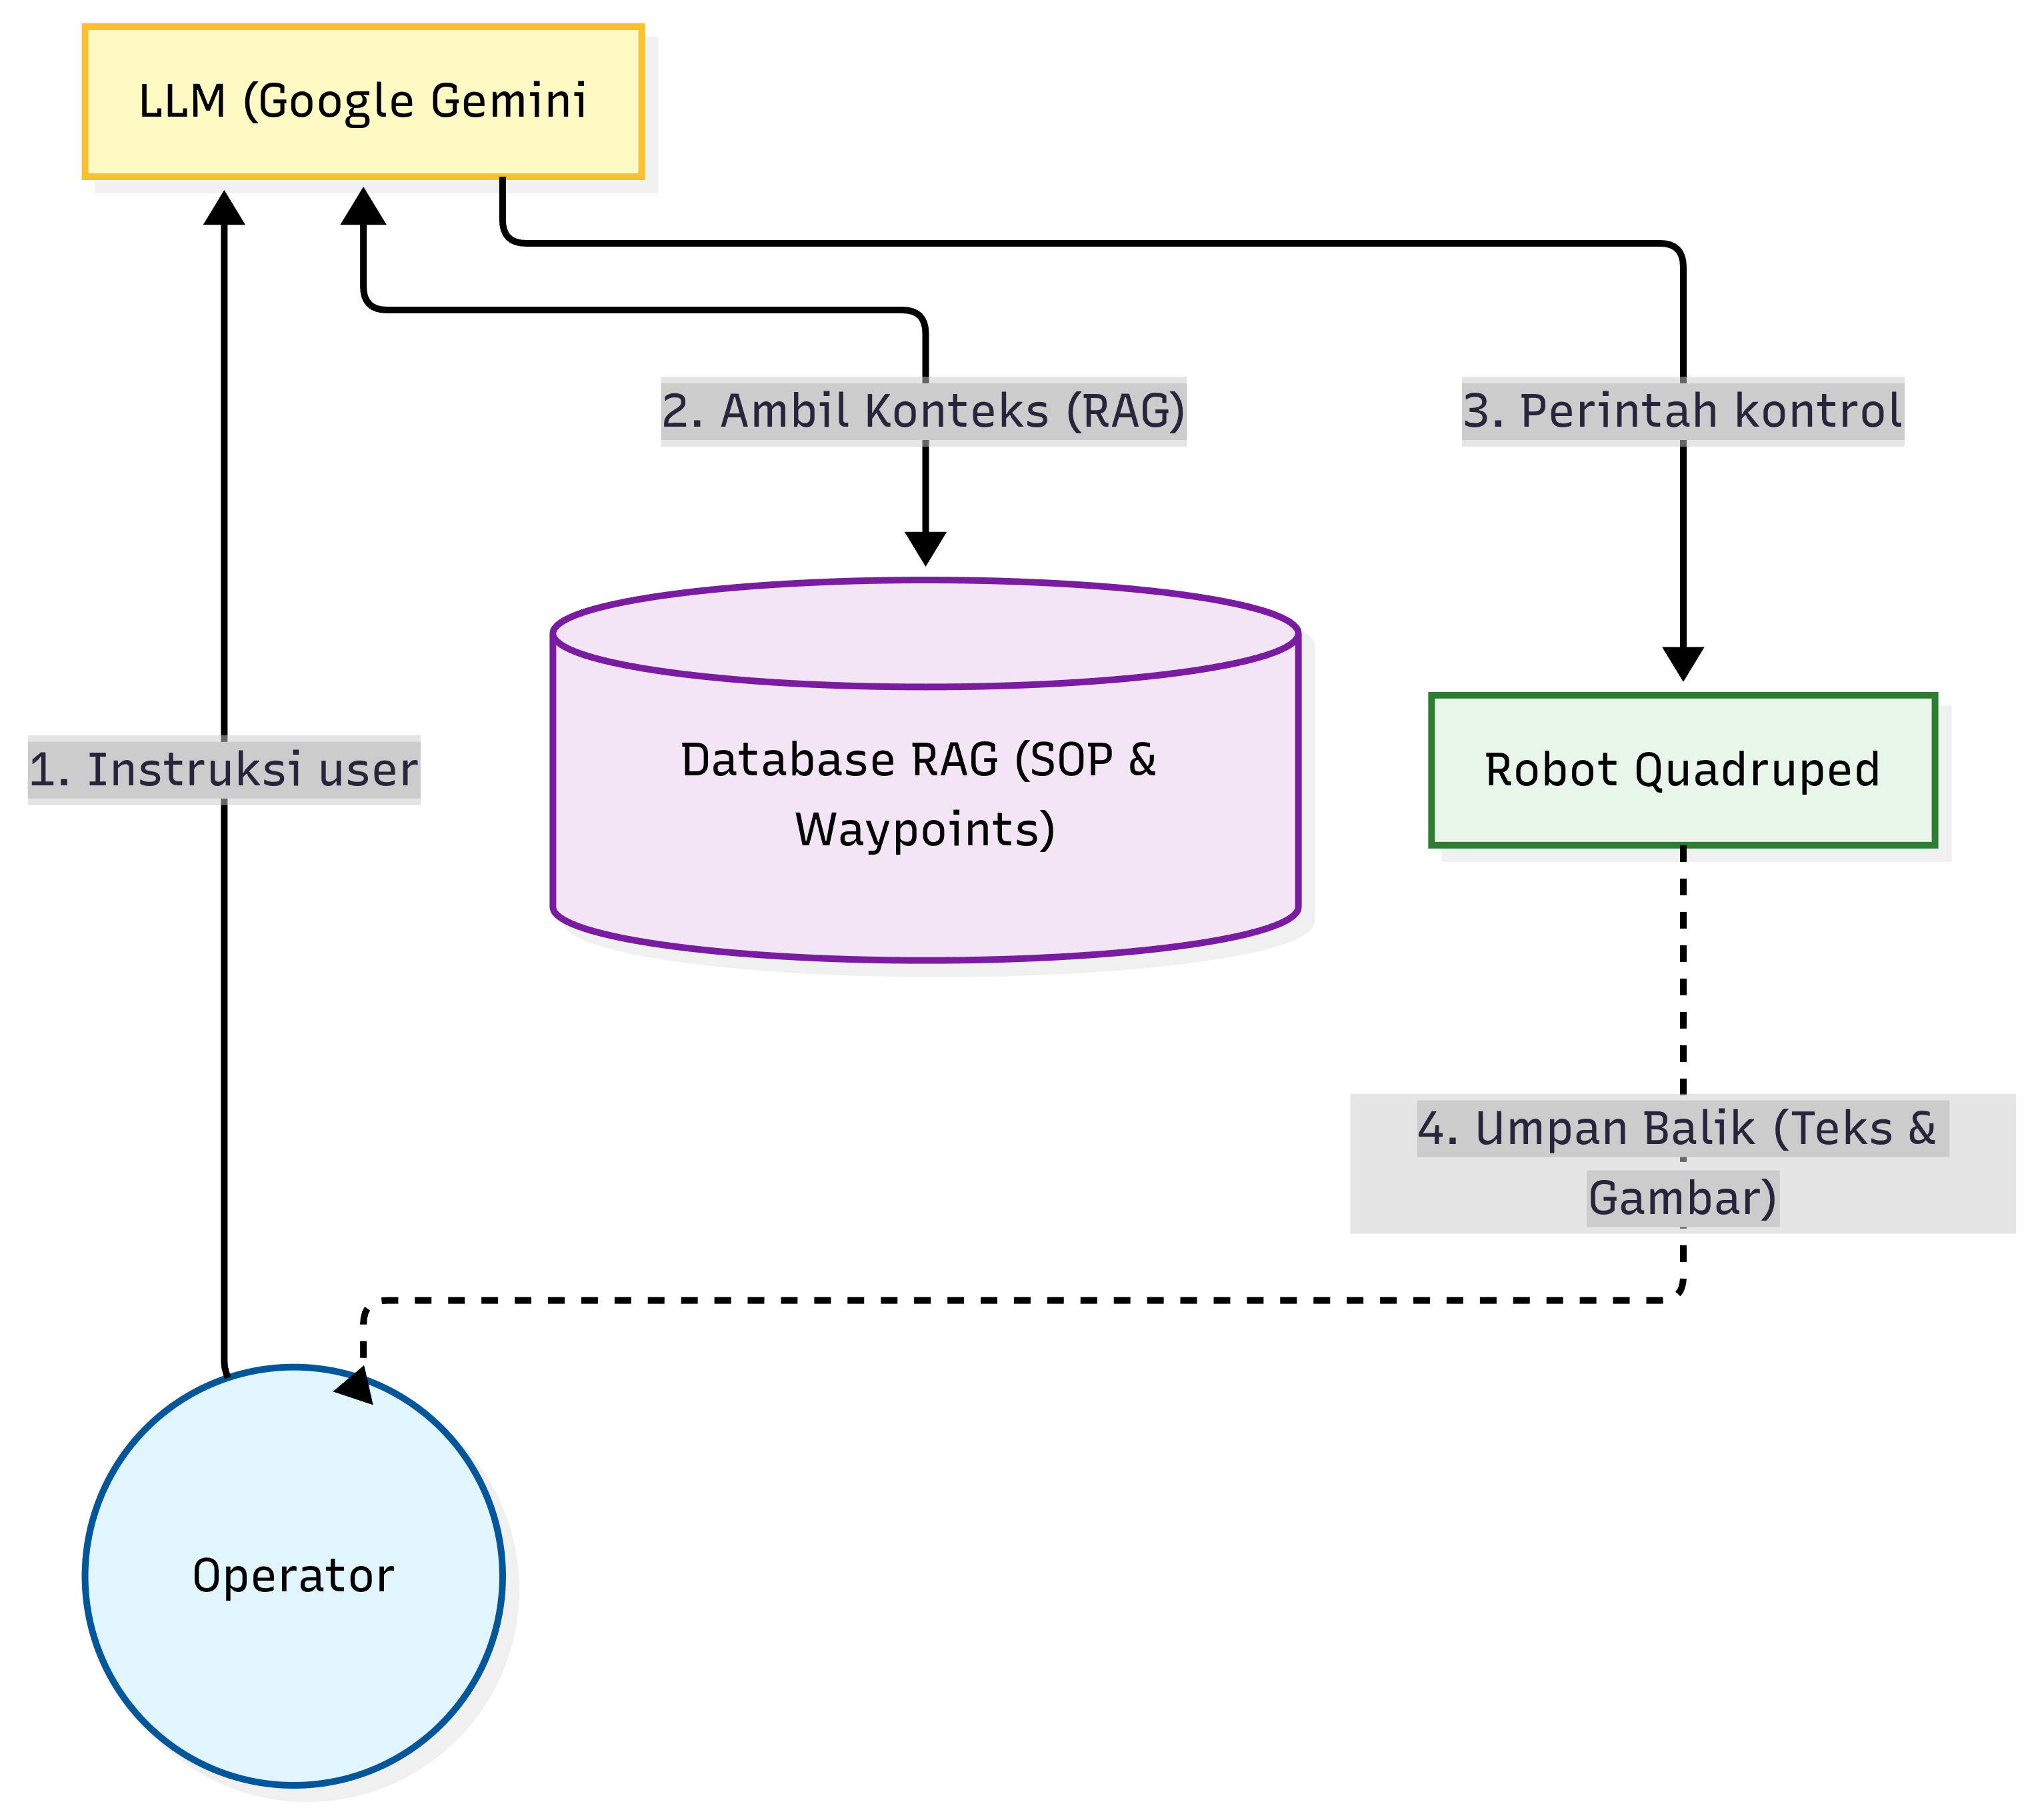
\includegraphics[width=0.5\textwidth]{Init/gambar/umum.png} 
    \caption{Diagram Umum Sistem}
    \label{fig:high_level_diagram}
\footnotesize \textbf{Sumber:} Dokumentasi Penulis
\end{figure}

Mekanisme kerja sistem diawali dengan pemberian instruksi oleh operator menggunakan bahasa alami, tanpa perlu mengetahui koordinat spesifik lokasi inspeksi. Perintah abstrak ini kemudian diproses oleh LLM (Google Gemini), namun tidak langsung diterjemahkan secara harfiah. Sistem terlebih dahulu melakukan (\textit{Context Retrieval}) ke basis data eksternal untuk mengambil informasi pendukung yang relevan, seperti peta semantik, titik koordinat waypoints, serta dokumen \textit{Standard Operating Procedure} (SOP) yang berkaitan dengan objek inspeksi. Langkah ini krusial untuk memastikan bahwa keputusan yang diambil oleh LLM didasarkan pada data spasial dan prosedural yang akurat, bukan sekadar halusinasi model bahasa.

Setelah pemahaman kontekstual terbentuk, LLM membangkitkan serangkaian perintah navigasi dan kontrol yang dapat dipahami oleh sistem kendali robot. Perintah ini dikirimkan ke robot \textit{quadruped} untuk dieksekusi, menggerakkan aktuator fisik menuju lokasi target secara otonom. Berbeda dengan pendekatan otomasi tradisional yang bersifat satu arah, sistem ini menerapkan mekanisme umpan balik interaktif. Setelah menyelesaikan suatu aksi navigasi atau pengambilan data, robot secara proaktif mengirimkan laporan status beserta bukti visual kembali kepada operator. Mekanisme \textit{Human-in-the-Loop} ini memberikan kesempatan bagi operator untuk memvalidasi hasil tindakan robot sebelum melanjutkan ke tahap berikutnya, sehingga menjamin keamanan dan adaptabilitas operasi inspeksi di lingkungan yang dinamis.

\subsection{Arsitektur Sistem}
Arsitektur sistem dalam penelitian ini menggunakan pendekatan terdistribusi yang mengintegrasikan kemampuan penalaran tingkat tinggi dari \textit{Large Multimodal Model} (LMM) dengan sistem kendali robotik. Komponen-komponen sistem dirancang secara modular dan saling terhubung melalui jaringan TCP/IP lokal maupun internet. Gambaran menyeluruh mengenai arsitektur sistem dan topologi data disajikan pada Gambar \ref{fig:arsitektur_sistem}.

\begin{figure}[H]
    % Pastikan diagram mermaid baru sudah di-export jadi gambar
    \centering
    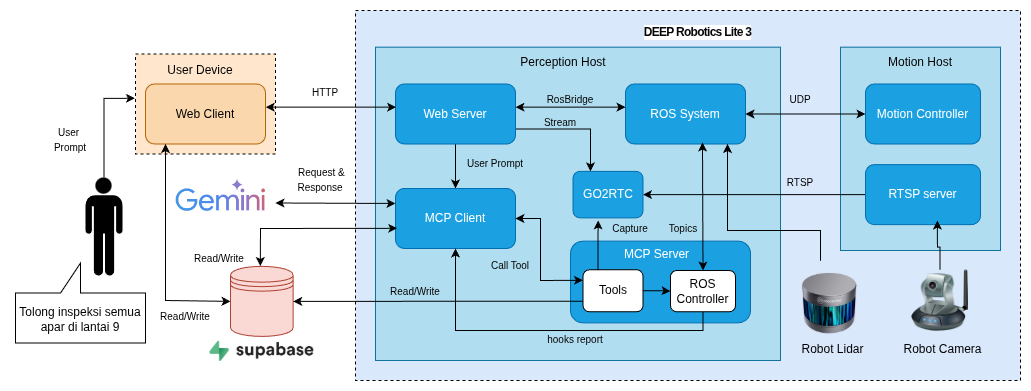
\includegraphics[width=1.0\textwidth]{Init/gambar/arsitektur_new.png}
    \caption{Diagram Arsitektur Sistem}
    \label{fig:arsitektur_sistem}
    \footnotesize \textbf{Sumber:} Dokumentasi Penulis
\end{figure}


\subsubsection{Google Gemini API}

Google Gemini API merupakan komponen yang berperan sebagai otak untuk sistem inspeksi. Gemini berfungsi untuk memahami perintah bahasa alami dari operator yang dikirim melalui \textit{Web Client}. Perintah tersebut dianalisis untuk membuat rencana inspeksi. Gemini menggunakan fitur \textit{function calling} untuk mengakses berbagai \textit{tools} yang ada pada MCP Server. Dengan fitur ini, Gemini bisa memutuskan kapan harus menggerakkan robot, kapan harus mengambil foto, atau kapan harus mencari dokumen SOP di \textit{database}. Gemini API juga berperan dalam proses analisis visual pada saat inspeksi berlangsung. Ketika kamera robot menangkap \textit{image} sebuah objek, \textit{image} tersebut dikirim ke Gemini API bersamaan dengan instruksi dari dokumen SOP. Gemini akan membandingkan kondisi visual objek pada foto dengan standar yang tertulis di SOP.

\subsubsection{Supabase}

Supabase dalam sistem ini berperan sebagai platform \textit{Backend-as-a-Service} (BaaS). Komponen ini berfungsi sebagai pusat penyimpanan data yang digunakan oleh \textit{Web Client}, \textit{MCP Client}, dan \textit{MCP Server}. Fungsi pertama dari Supabase adalah sebagai \textit{database} relasional. Di dalam \textit{database} ini, sistem menyimpan daftar lokasi dan koordinat target. Selain itu, Supabase juga menyimpan \textit{Session History} yang berisi riwayat percakapan antara operator dan Gemini agar konteks misi sebelumnya tetap terjaga. Fungsi kedua adalah sebagai \textit{Storage} untuk menyimpan dokumen dan \textit{image}. Supabase Storage digunakan untuk menyimpan file dokumen SOP, serta setiap foto yang diambil oleh kamera robot saat proses inspeksi.

\subsubsection{Web App}

\textit{Web App} merupakan antarmuka utama yang digunakan oleh operator untuk mengendalikan dan memantau robot. Komponen ini dijalankan di dalam PC internal robot. Komponen ini berfungsi sebagai media komunikasi antara operator dan \textit{AI Agent} melalui panel \textit{chat}. Selain itu, \textit{Web App} juga menyediakan fitur manajemen data untuk mengatur lokasi \textit{waypoint} target dan untuk mengelola file panduan inspeksi. Fungsi lainnya dari \textit{Web App} adalah sebagai pusat monitoring \textit{real-time}. Operator dapat melihat \textit{video feed} dari kamera robot secara langsung melalui protokol WebRTC dan data telemetri robot melalui koneksi \textit{Rosbridge WebSocket}.

\subsubsection{MCP Client }
Komponen ini berfungsi sebagai penghubung antara antarmuka web, Gemini API, dan MCP Server dalam menjalankan mekanisme \textit{Agentic Loop}. Ketika Gemini memutuskan untuk menjalankan suatu tindakan melalui fitur \textit{function calling}, MCP Client akan menerima permintaan tersebut dan meneruskannya ke \textit{tools} yang sesuai pada MCP Server. Setelah memperoleh respons, MCP Client akan mengirimkan kembali hasil tersebut kepada Gemini. MCP Client juga mengelola riwayat percakapan dengan menyimpan data interaksi ke dalam \textit{database}. Selain itu, MCP Client bertanggung jawab dalam mengelola \textit{System Prompt} yang berisi konfigurasi kepribadian serta batasan operasional yang harus dipatuhi oleh Gemini selama menjalankan misi.

\subsubsection{MCP Server}
MCP Server beroperasi sebagai lapisan abstraksi lokal yang bertugas mengekspos seluruh fungsionalitas robot menjadi kumpulan \textit{tools}. Server ini bertugas mendengarkan perintah pemanggilan \textit{tools} dari agen AI melalui MCP Client. Perannya sangat esensial karena tools yang ada pada MCP Server tersebut yang akan menggerakkan robot dengan memanfaatkan fungsionalitas yang ada pada ROS. Selain menggerakan robot, pencarian koordinat \textit{waypoint} objek target, pengambilan \textit{image} dari kamera robot, pengambilan dokumen SOP dari basis data, serta analisis \textit{image} dilakukan oleh komponen ini melalui \textit{tools}-nya. MCP server juga bertanggung jawab dalam melakukan mekanisme webhook untuk mengirimkan status ke MCP Client setelah pergerakan robot selesai.

\subsubsection{Sistem ROS}

ROS berperan sebagai sistem yang mengelola seluruh komunikasi dan tugas navigasi pada robot. Sistem ini memproses data mentah dari \textit{Robot Lidar} untuk menghasilkan peta lingkungan serta menentukan posisi koordinat robot secara akurat selama misi berlangsung. Seluruh koordinasi pergerakan fisik dikelola melalui koneksi UDP menuju \textit{Motion Host}. Untuk menjembatani komunikasi dengan antarmuka luar, \textit{RosBridge} digunakan sebagai penyedia \textit{WebSocket} yang memungkinkan web mengakses data telemetri robot. Integrasi ROS dengan MCP Server dilakukan melalui mekanisme \textit{topics} yang memungkinkan tools pada MCP server untuk dapat mengakses fungsionalitas ROS. 

\subsubsection{Motion Controller}
\textit{Motion Controller} merupakan unit kontrol tingkat terendah yang berinteraksi langsung dengan perangkat keras robot Jueying Lite3. Subsistem ini memegang kendali atas keseimbangan dinamis robot dan rotasi sendi-sendi aktuator kaki (\textit{gait planning}). Modul ini bertugas mengubah perintah kecepatan abstrak (\textit{velocity command}) dari ROS menjadi sinyal torsi motor yang secara fisik menggerakkan robot.

\subsubsection{GO2RTC}
GO2RTC merupakan komponen penyedia layanan \textit{streaming} video yang bertugas mengelola distribusi data visual dari kamera robot menuju berbagai modul dalam sistem. Komponen ini menerima aliran data melalui protokol RTSP dari \textit{RTSP server} yang terhubung langsung dengan perangkat keras kamera pada \textit{Motion Host}. 

\subsubsection{RTSP Server}

RTSP server beroperasi di dalam modul \textit{Motion Host} sebagai penyedia akses data visual mentah yang bersumber langsung dari kamera robot. Komponen ini memiliki tanggung jawab untuk mengelola aliran data video dan menyediakannya dalam format standar melalui protokol \textit{Real-Time Streaming Protocol}.

\subsection{Alur Sistem}

Alur kerja dari sistem inspeksi visual otonom ini dibagi menjadi tiga fase utama, yaitu fase perencanaan, fase eksekusi dan analisis, serta fase pelaporan hasil dan interaksi manusia. Interaksi data dan kendali antar komponen sistem melibatkan operator, AI Agent yang bertindak sebagai MCP Client dan terintegrasi dengan Gemini, MCP Server, database Supabase, serta robot quadruped yang menjalankan ROS dan kamera. Seluruh komponen ini bekerja secara sinkron melalui pertukaran pesan dan pemanggilan fungsi untuk memastikan misi inspeksi dapat berjalan dengan aman dan terarah.

\begin{figure}[H]
    \centering
    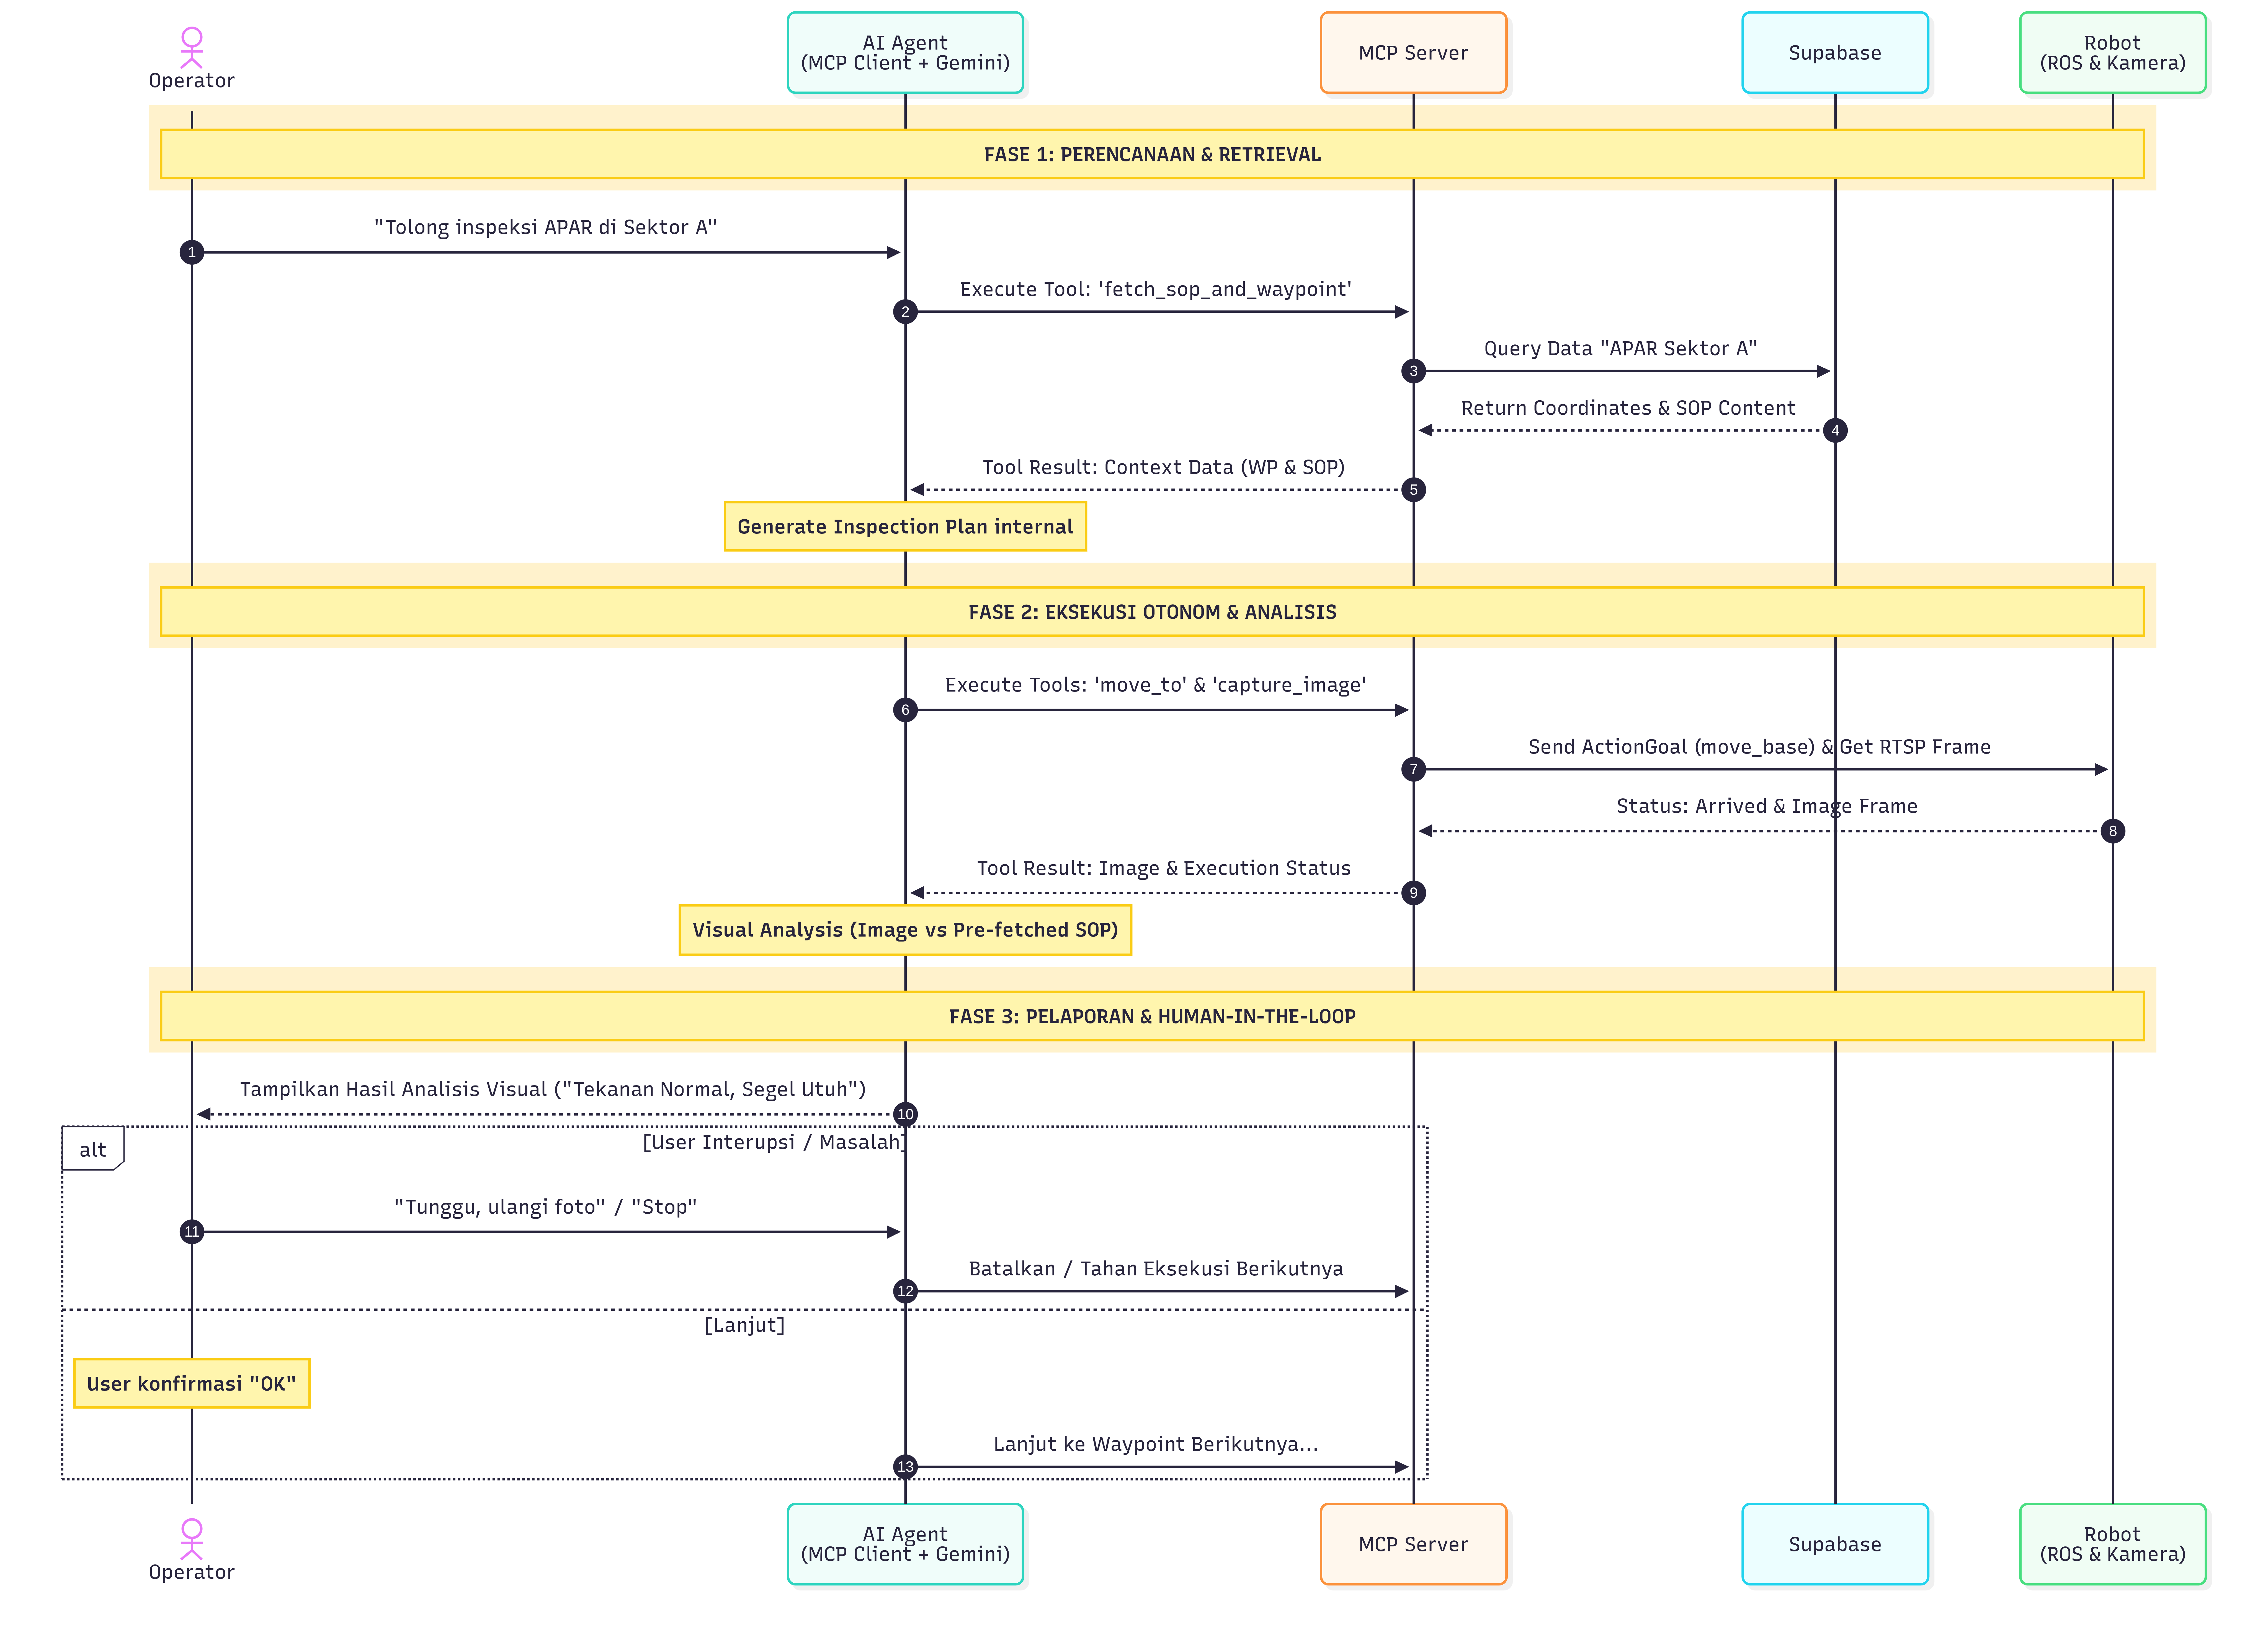
\includegraphics[width=1.0\textwidth]{Init/gambar/alur.png}
    \caption{Diagram Sekuensial Alur Interaksi Sistem}
    \label{fig:sequence_diagram}
\footnotesize \textbf{Sumber:} Dokumentasi Penulis
\end{figure}

\subsubsection{Fase Perencanaan}

Fase pertama berfokus pada penerimaan instruksi dari operator dan penyusunan rencana kerja oleh AI Agent sebelum robot melakukan pergerakan fisik. Proses ini dimulai ketika operator memasukkan perintah dalam bentuk bahasa alami melalui fitur chat pada web dashboard untuk memeriksa objek tertentu pada lokasi spesifik. AI Agent kemudian menerima pesan tersebut lalu mengidentifikasi kebutuhan informasi tambahan dan mengirimkan permintaan kepada MCP Server untuk memanggil fungsi pencarian dokumen SOP serta data koordinat tujuan atau waypoint. Selanjutnya, MCP Server melakukan query data ke database Supabase untuk mengambil data koordinat objek dan isi dokumen SOP yang relevan dengan instruksi operator. 

Database Supabase mengembalikan data koordinat serta konten SOP yang dicari kepada MCP Server untuk kemudian diteruskan kembali ke AI Agent. Setelah menerima data tersebut, AI Agent memproses informasi untuk menyusun sebuah rencana inspeksi visual secara mandiri berdasarkan prioritas urutan lokasi objek terdekat. Rencana inspeksi yang telah matang dikirimkan oleh AI Agent ke halaman web dashboard untuk ditampilkan kepada operator. Pada akhir fase ini, operator membaca rencana tersebut dan memberikan konfirmasi persetujuan melalui input chat sebagai bentuk kendali Human-in-the-Loop sebelum sistem masuk ke tahap berikutnya.

\subsubsection{Fase Eksekusi dan Analisis}

Setelah rencana kerja disetujui oleh operator, sistem masuk ke fase kedua untuk menggerakkan robot dan melakukan analisis visual pada objek target. Langkah awal dimulai saat AI Agent memberikan perintah eksekusi kepada MCP Server untuk menjalankan \textit{tool} navigasi ke titik objek pertama. MCP Server menerjemahkan perintah tersebut menjadi pesan ROS lalu mengirimkannya ke ROS Navigation Stack pada komputer internal robot sekaligus mengirimkan status bahwa proses navigasi sedang berjalan kepada AI Agent. Robot kemudian bergerak secara otonom menuju koordinat target dan mengirimkan laporan status kepada MCP Server setelah sistem navigasi robot sampai di titik tujuan. 

MCP Server mendeteksi status kedatangan tersebut lalu mengirimkan laporan balik menggunakan mekanisme webhook kepada AI Agent. Setelah menerima laporan tersebut, AI Agent memerintahkan MCP Server untuk menjalankan \textit{tool} pengambilan \textit{image} dan analisis objek visual. MCP Server segera mengakses kamera robot untuk mengambil \textit{image} snapshot dari objek di depannya. Kamera robot menangkap \textit{image} lalu mengirimkan file \textit{image} tersebut kembali ke MCP Server untuk dianalisis secara visual dengan membandingkan kondisi riil pada \textit{image} terhadap poin aturan yang ada di dalam dokumen SOP menggunakan model multimodal Gemini. Setelah analisis selesai, MCP Server menyimpan file \textit{image} hasil tangkapan kamera ke dalam Supabase Storage. Terakhir, MCP Server mengembalikan respons berupa URL \textit{image} dan teks hasil analisis visual kepada AI Agent.

\subsubsection{Fase Pelaporan}

Fase terakhir merupakan tahap pelaporan hasil kerja robot kepada operator serta penentuan langkah keberlanjutan sistem. Proses ini diawali dengan AI Agent menampilkan hasil analisis visual beserta foto objek dari lapangan ke panel chat web dashboard agar dapat diperiksa oleh operator. Pada tahap ini, sistem menyediakan percabangan melanjutkan rencana inspeksi atau intervensi langsung dari operator. 

Jika operator memberikan pesan interupsi karena melihat adanya keanehan atau memerlukan tindakan lebih lanjut, AI Agent akan langsung merespons pesan tersebut dan meminta MCP Server mengeksekusi \textit{tool} sesuai perintah baru dari operator. Sebaliknya, jika kondisi dinilai aman dan operator memberikan konfirmasi untuk lanjut, AI Agent akan memerintahkan MCP Server untuk menggerakkan robot menuju ke titik koordinat atau waypoint berikutnya sesuai dengan daftar rencana awal yang telah disusun sebelumnya.

% \subsection{Alur Interaksi Sistem}
% Gambar \ref{fig:sequence_diagram} mengilustrasikan alur kerja sistem dalam menangani misi inspeksi. Alur sistem ini dibagi menjadi tiga fase utama, yaitu perencanaan, eksekusi otonom, dan pelaporan. Fase pertama diawali saat Operator memberikan instruksi bahasa alami melalui antarmuka web yang kemudian diteruskan ke \textit{AI Agent}. Untuk menyusun rencana, agen tidak mengakses basis data secara langsung, melainkan mengeksekusi pemanggilan fungsi (\textit{tool execution}) ke \textit{MCP Server}. \textit{MCP Server} bertugas melakukan kueri ke basis data \textit{Supabase} untuk mengambil konteks tugas spesifik, yaitu koordinat \textit{waypoint} dan dokumen \textit{Standard Operating Procedure} (SOP). Pendekatan \textit{Agentic RAG} memastikan bahwa rencana inspeksi yang dihasilkan oleh model LLM selalu berlandaskan pada data yang valid.

% Fase kedua dijalankan setelah persetujuan Operator diterima, \textit{AI Agent} menginstruksikan \textit{MCP Server} untuk menjalankan perintah aksi seperti navigasi dan pengambilan data visual. Di dalam \textit{Perception Host} robot, \textit{MCP Server} menerjemahkan perintah ini menjadi \textit{Action Goal} yang kemudian didistribusikan ke \textit{Navigation Stack} pada sistem ROS. Begitu robot mengonfirmasi kedatangannya di titik target, server akan mengekstrak gambar  dari Kamera. Gambar beserta status eksekusi dikembalikan ke \textit{AI Agent}, yang kemudian melakukan penalaran visual dengan membandingkan kondisi aktual objek terhadap parameter ideal yang diuraikan dalam dokumen SOP.

% Pada fase ketiga, hasil analisis visual disajikan kepada Operator. Di titik inilah mekanisme intervensi HITL memegang peranan krusial. Operator memiliki otoritas penuh untuk memvalidasi temuan AI; jika terdeteksi anomali atau sudut pandang kamera kurang jelas, Operator dapat memberikan interupsi untuk meminta pengambilan ulang foto atau menghentikan pergerakan. Jika hal ini terjadi, \textit{MCP Server} akan segera membatalkan atau menangguhkan eksekusi selanjutnya. Sebaliknya, apabila Operator mengonfirmasi temuan tersebut, sistem akan melanjutkan rencana inspeksi ke \textit{waypoint} berikutnya secara berkesinambungan.



\subsection{Desain Antarmuka}
Antarmuka pengguna (\textit{User Interface}) pada sistem ini dirancang berbasis web modern untuk memberikan pengalaman interaksi \textit{Human-in-the-Loop} yang intuitif dan responsif. Aplikasi antarmuka ini bertindak sebagai \textit{front-end} dari MCP Client yang menghubungkan operator dengan logika agen cerdas dan umpan balik visual dari robot. Rancangan visual sistem dibagi menjadi tiga modul utama yaitu Pusat Kendali, Manajemen Pengetahuan, dan Riwayat Sesi.

\subsubsection{Halaman Pusat Kendali}
Halaman ini merupakan ruang kerja utama operator yang dirancang dengan tata letak layar terbagi (\textit{split-screen}) untuk memfasilitasi pengawasan visual dan kontrol tekstual secara simultan. Sebagaimana diperlihatkan pada Gambar \ref{fig:ui_command_center}, panel sebelah kiri didedikasikan untuk \textit{Visual Monitor} yang menampilkan aliran video \textit{real-time} dari kamera robot melalui protokol WebRTC. Di atas tampilan video, terdapat lapisan informasi (\textit{overlay}) telemetri yang memberikan data kritis seperti status operasional robot, persentase baterai, kekuatan sinyal jaringan, dan kecepatan gerak linier.

\begin{figure}[h!]
    \centering
    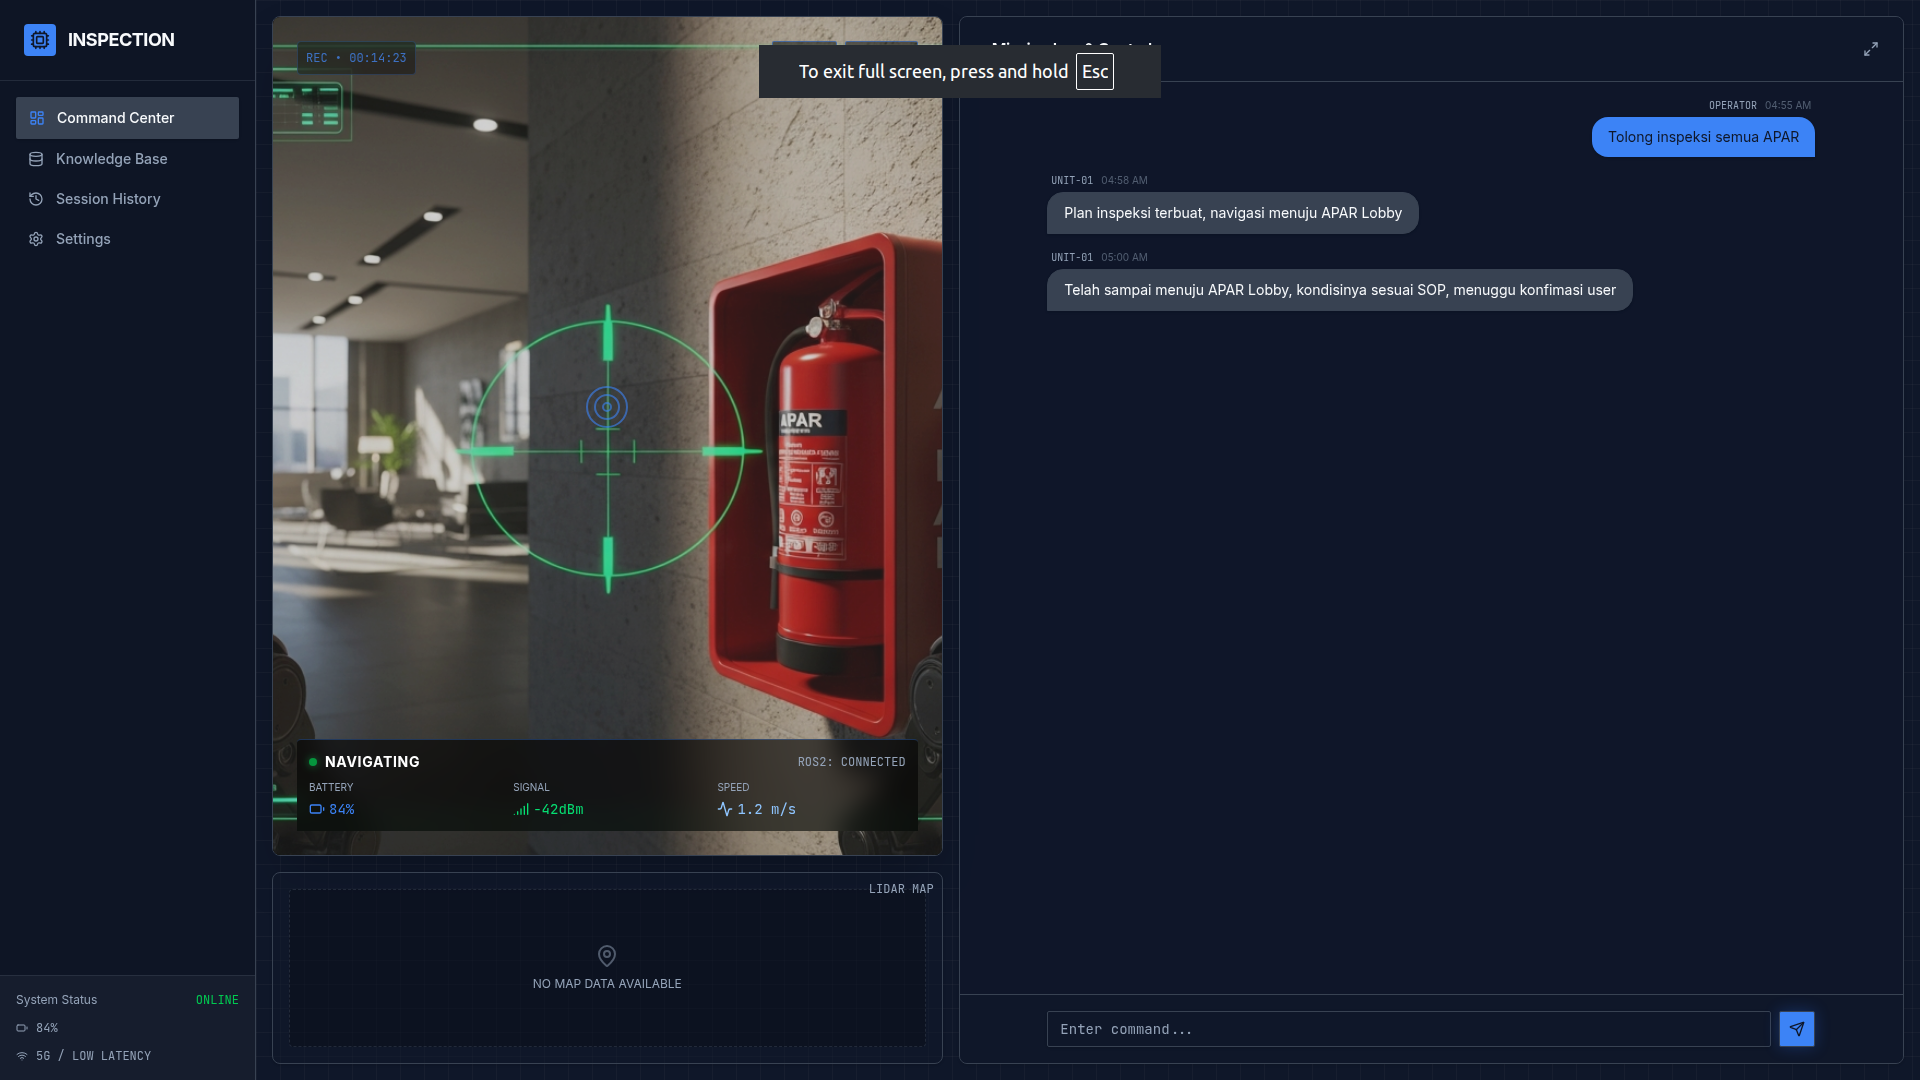
\includegraphics[width=0.8\textwidth]{Init/gambar/ui_command_center.png} % Ganti dengan nama file screenshot Command Center
    \caption{Rancangan Antarmuka Pusat Kendali}
    \label{fig:ui_command_center}
\footnotesize \textbf{Sumber:} Dokumentasi Penulis
\end{figure}

Panel sebelah kanan berfungsi sebagai antarmuka percakapan yang menjadi saluran komunikasi utama antara manusia dan agen AI. Desain panel ini mengadopsi gaya aplikasi pesan instan modern di mana instruksi operator ditampilkan di sisi kanan, sementara respons agen dan laporan inspeksi ditampilkan di sisi kiri. Mekanisme ini memungkinkan operator untuk memberikan perintah kompleks (contoh: "Tolong inspeksi semua APAR") dan menerima konfirmasi langkah demi langkah dari robot tanpa perlu berpindah halaman, menjaga fokus operator tetap pada konteks misi yang sedang berjalan.

\subsubsection{Halaman Manajemen Pengetahuan}
Halaman ini berfungsi sebagai panel administrasi untuk mengelola data yang tersimpan di dalam basis data Supabase, yang menjadi fondasi bagi mekanisme \textit{Retrieval-Augmented Generation} (RAG). Antarmuka ini memisahkan pengelolaan data menjadi dua tabulasi utama. Tabulasi pertama, seperti terlihat pada Gambar \ref{fig:ui_waypoints}, adalah manajemen \textit{Waypoints} yang menampilkan daftar lokasi inspeksi dalam bentuk tabelar. Operator dapat memantau koordinat spasial ($x, y, z$), status aktif lokasi, dan melakukan penyuntingan data tanpa perlu menulis kueri SQL manual. Tabulasi kedua difokuskan pada pengelolaan dokumen prosedur standar (SOP). Antarmuka ini menyediakan fitur pengunggahan berkas (\textit{drag-and-drop}) untuk dokumen yang akan dijadikan referensi verifikasi oleh agen cerdas.

\begin{figure}[h]
    \centering
    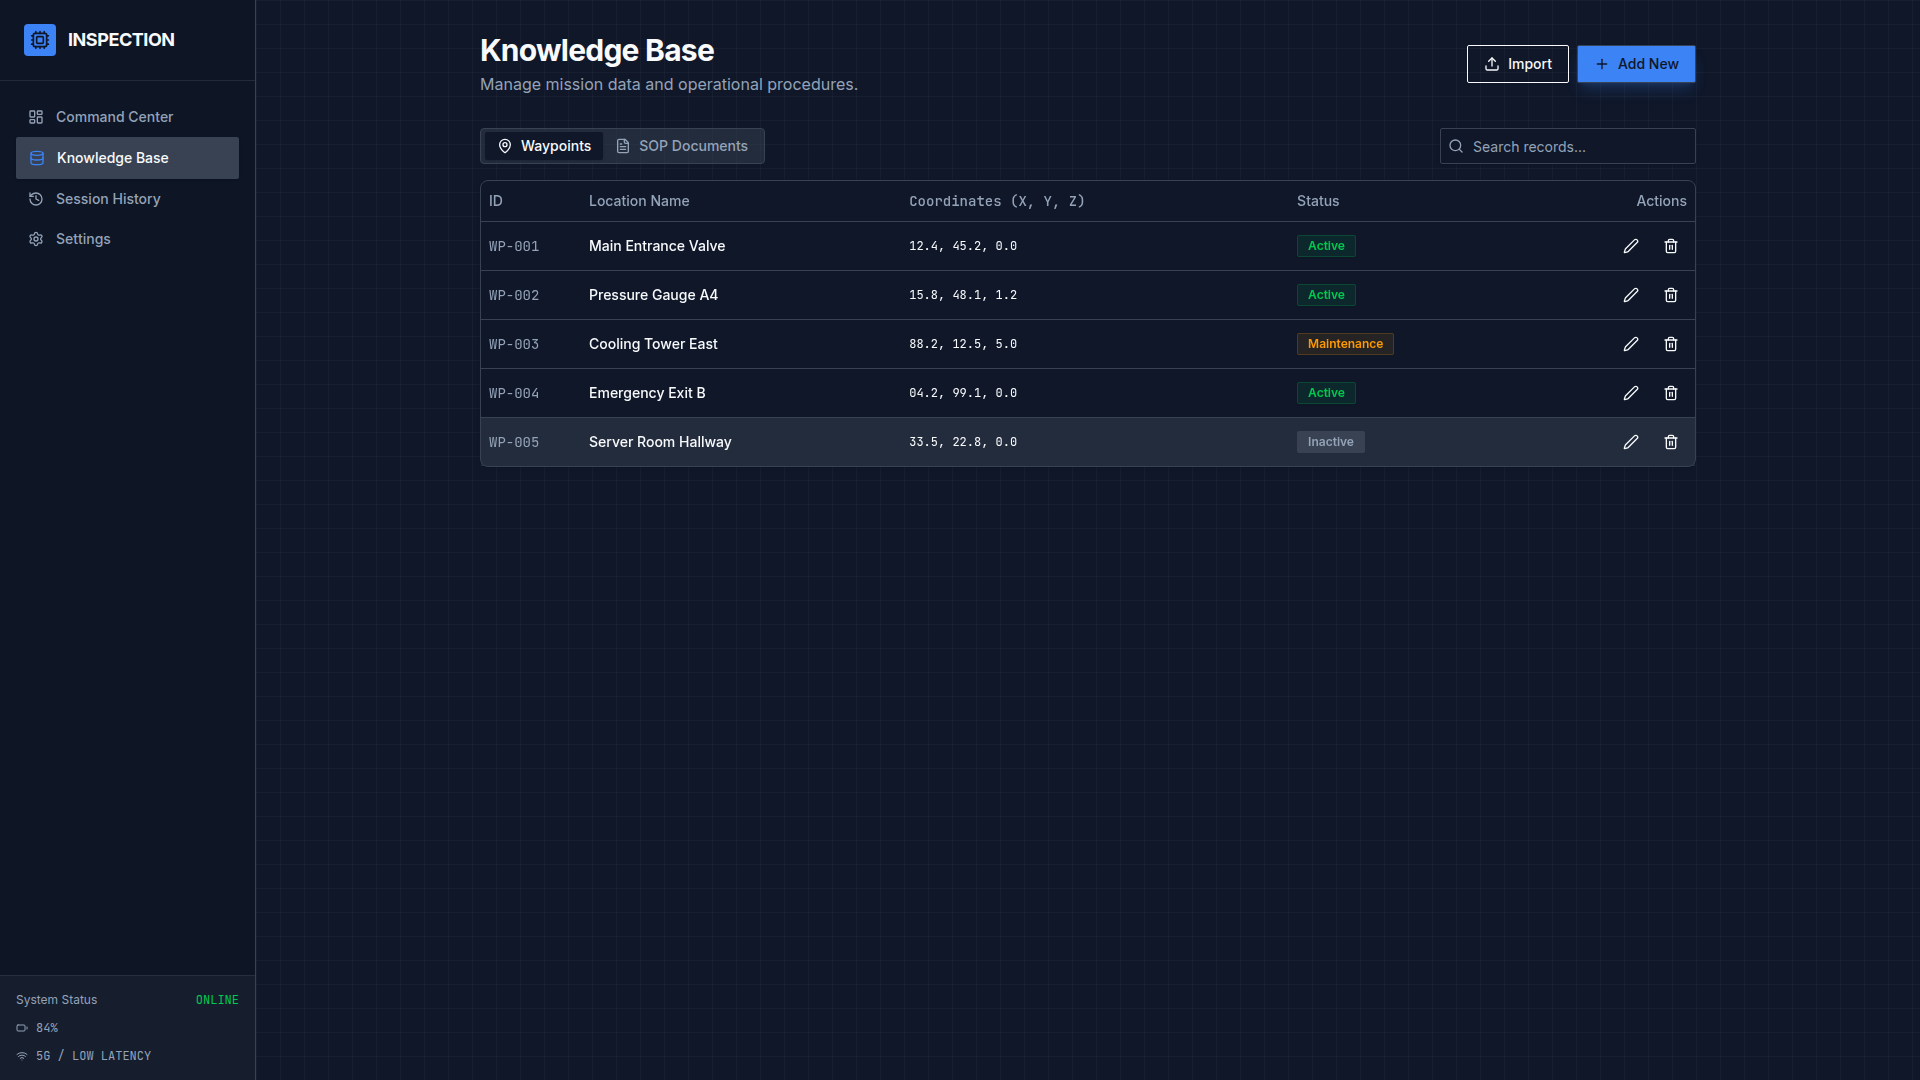
\includegraphics[width=0.8\textwidth]{Init/gambar/ui_waypoints.png} % Ganti dengan nama file screenshot Waypoints
    \caption{Antarmuka Manajemen Data Waypoint Inspeksi}
    \label{fig:ui_waypoints}
\footnotesize \textbf{Sumber:} Dokumentasi Penulis
\end{figure}

\begin{figure}[H]
    \centering
    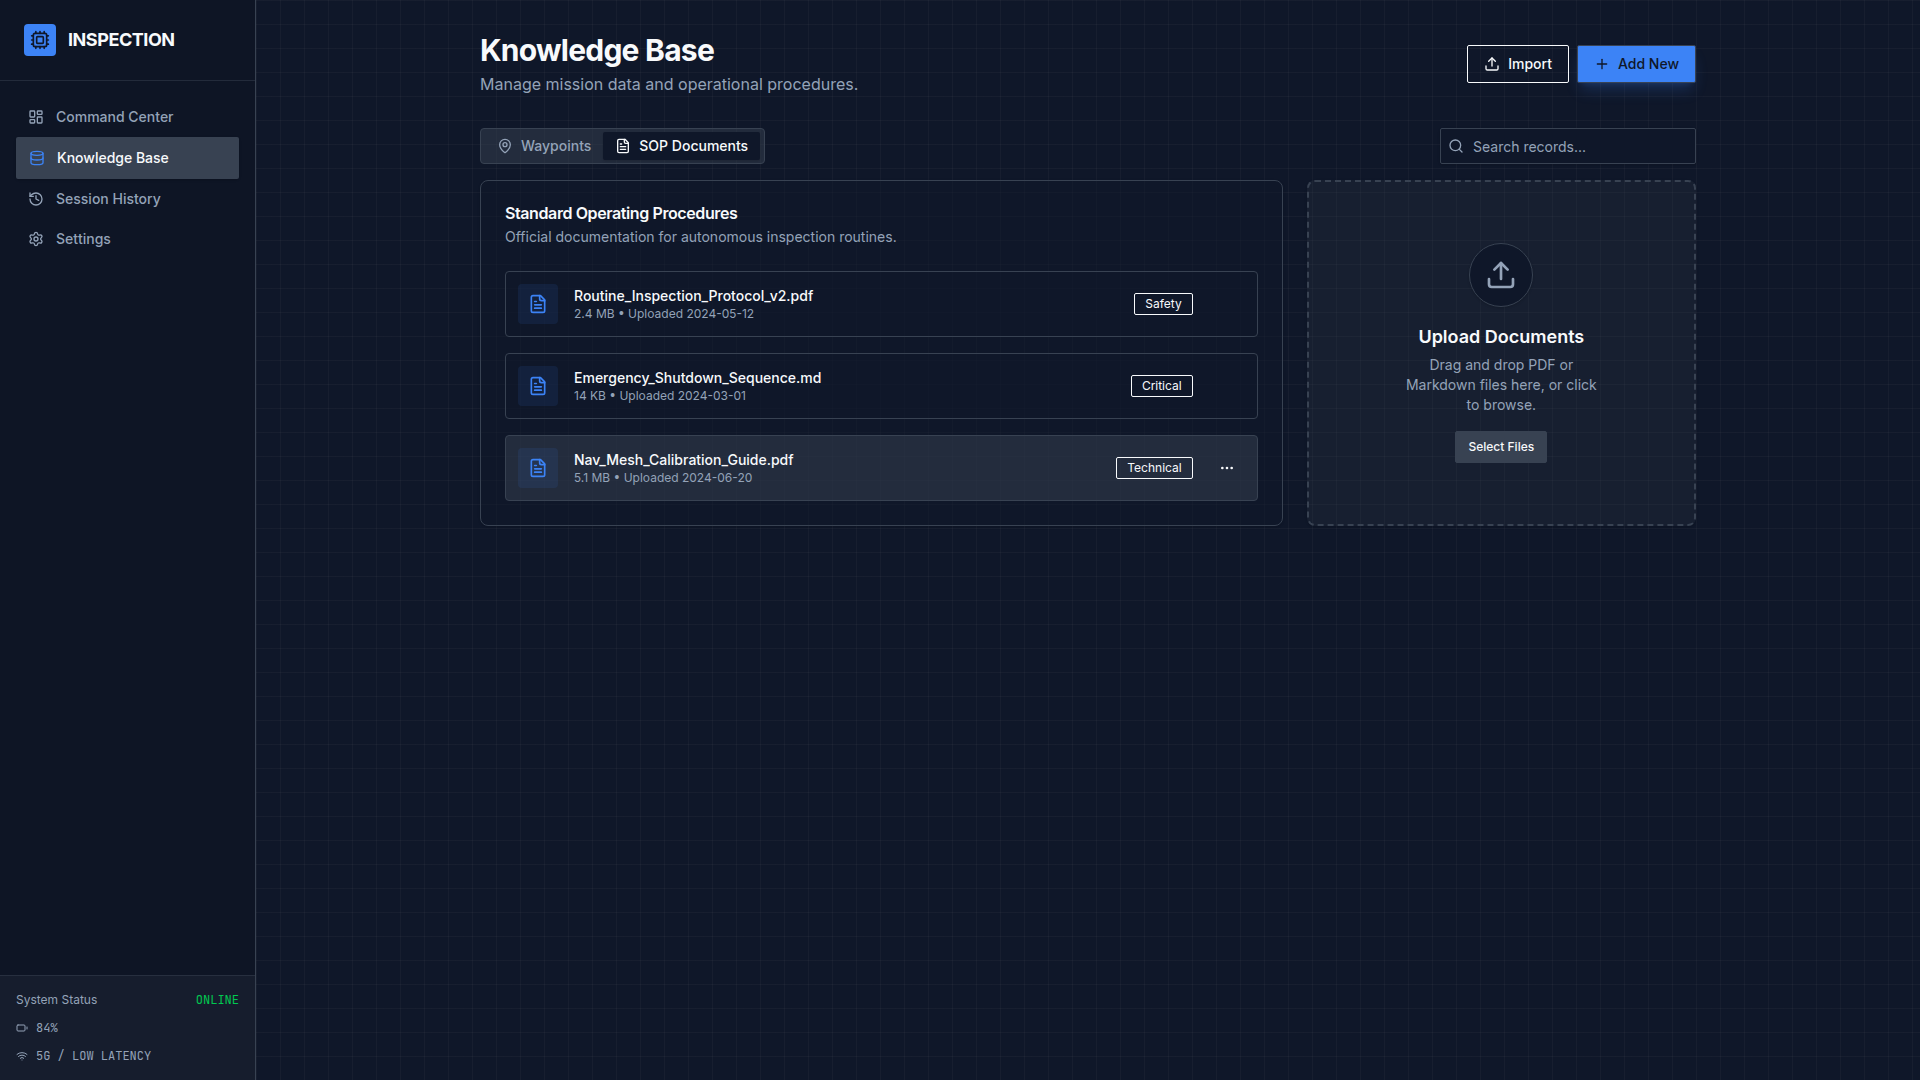
\includegraphics[width=0.8\textwidth]{Init/gambar/ui_sop.png} % Ganti dengan nama file screenshot Waypoints
    \caption{Antarmuka Manajemen File SOP}
    \label{fig:ui_sop}
\footnotesize \textbf{Sumber:} Dokumentasi Penulis
\end{figure}



% \subsection{Desain Perangkat Keras}
% \subsubsection{Spesifikasi Perangkat Keras}

% Platform robot yang digunakan dalam penelitian ini adalah Jueying Lite3 Pro yang diproduksi oleh DEEPRobotics (Hangzhou Yunshenchu Technology Co., Ltd.). Robot ini merupakan varian \textit{base} dari seri Lite3 yang tidak dilengkapi sensor LiDAR secara bawaan. Dalam penelitian ini, sensor LiDAR Leishen C16 dipasang secara terpisah sebagai perangkat tambahan sehingga konfigurasi akhir robot setara dengan varian Jueying Lite3 LiDAR \cite{DEEPRoboticsLite3Pro2024}.

% Secara fisik, robot memiliki 12 derajat kebebasan (DOF) dengan distribusi tiga sendi aktif per kaki, yaitu HipX, HipY, dan Knee. Bobot total robot mencapai 12,7~kg termasuk baterai. Pada posisi berdiri penuh, dimensi robot adalah 610 $\times$ 370 $\times$ 445~mm, sedangkan saat dalam posisi duduk atau istirahat ukurannya menjadi 680 $\times$ 370 $\times$ 175~mm. Robot mampu melewati kemiringan hingga 40° dan rintangan setinggi 15~cm, menjadikannya cocok untuk digunakan di area industri yang memiliki variasi kontur lantai. Baterai berkapasitas 4,4~Ah dengan tegangan nominal 28,8~V mampu menopang operasi robot selama 1,5 hingga 2 jam tanpa muatan tambahan. Spesifikasi dimensi dan mekanik selengkapnya disajikan pada Tabel~\ref{tab:spek-mekanik}.

% \begin{table}[h!]
% \centering
% \caption{Spesifikasi dimensi dan mekanik Jueying Lite3 Pro \cite{DEEPRoboticsLite3Pro2024}}
% \label{tab:spek-mekanik}
% \begin{tabular}{|l|l|l|}
% \hline
% \textbf{Parameter} & \textbf{Nilai} & \textbf{Keterangan} \\ \hline
% Ukuran berdiri (P $\times$ L $\times$ T) & 610 $\times$ 370 $\times$ 445 mm & Posisi berdiri normal \\ \hline
% Ukuran duduk (P $\times$ L $\times$ T) & 680 $\times$ 370 $\times$ 175 mm & Posisi duduk/istirahat \\ \hline
% Berat total & 12,7 kg & Termasuk baterai \\ \hline
% Jumlah derajat kebebasan & 12 DOF & 3 sendi per kaki \\ \hline
% Kemampuan tanjakan & 40° & Sudut kemiringan maksimum \\ \hline
% Tinggi rintangan & 15 cm & Tinggi rintangan yang dapat dilalui \\ \hline
% Kapasitas baterai & 4,4 Ah / 28,8 V & — \\ \hline
% Durasi operasi & 1,5 -- 2 jam & Tanpa muatan tambahan \\ \hline
% \end{tabular}
% \end{table}

% Pada sisi komputasi, robot dilengkapi dengan \textit{AI Computer} berbasis NVIDIA Jetson Xavier NX yang menjalankan seluruh proses persepsi dan komputasi perangkat lunak, termasuk \textit{stack} navigasi ROS, MCP Server, dan MCP Client. Untuk sistem persepsi bawaan, robot memiliki satu kamera lebar (\textit{wide angle camera}) untuk pemantauan lingkungan, dua radar ultrasonik untuk deteksi rintangan jarak dekat, dan satu kamera kedalaman (\textit{depth camera}) untuk estimasi jarak objek. Sensor LiDAR Leishen C16 ditambahkan secara eksternal dan dipasang di bagian atas badan robot, menyediakan kemampuan pemindaian awan titik 3D 360° yang menjadi fondasi utama proses pemetaan dan lokalisasi \cite{DEEPRoboticsLite3LiDAR2025}. Spesifikasi sistem komputasi dan sensor selengkapnya disajikan pada Tabel~\ref{tab:spek-komputasi}.

% \begin{table}[h!]
% \centering
% \caption{Spesifikasi komputasi dan sensor Jueying Lite3 Pro}
% \label{tab:spek-komputasi}
% \begin{tabular}{|l|l|l|}
% \hline
% \textbf{Komponen} & \textbf{Spesifikasi} & \textbf{Fungsi} \\ \hline
% AI Computer & NVIDIA Jetson Xavier NX & Komputasi persepsi berbasis GPU \\ \hline
% Kamera lebar & Wide Angle Camera $\times$1 & Pemantauan lingkungan \\ \hline
% Radar ultrasonik & Ultrasonic Radar $\times$2 & Deteksi rintangan jarak dekat \\ \hline
% Kamera kedalaman & Depth Camera $\times$1 & Estimasi kedalaman objek \\ \hline
% LiDAR 3D (tambahan) & Leishen C16 & Pemetaan 3D dan lokalisasi \\ \hline
% \end{tabular}
% \end{table}

% \subsubsection{Arsitektur Perangkat Keras}

% Arsitektur perangkat keras sistem dirancang secara berlapis dengan memisahkan tanggung jawab antara unit komputasi, sensor, dan aktuator secara jelas. Gambar~\ref{fig:arsitektur_hardware} menyajikan gambaran menyeluruh mengenai topologi fisik dan aliran data antar-komponen dalam sistem.

% Komponen inti dari arsitektur ini adalah \textit{AI Computer} (NVIDIA Jetson Xavier NX) yang bertindak sebagai pusat komputasi tunggal robot. Semua proses perangkat lunak berjalan pada unit ini, mulai dari pembacaan data sensor LiDAR melalui \textit{driver} ROS, proses lokalisasi dan navigasi menggunakan \textit{Navigation Stack}, hingga layanan-layanan aplikasi seperti MCP Server dan MCP Client. Pemilihan arsitektur \textit{single-host} ini memungkinkan komunikasi antar-proses yang efisien melalui mekanisme \textit{inter-process communication} ROS tanpa memerlukan jaringan eksternal.

% Data sensorik mengalir dari LiDAR Leishen C16 ke Jetson Xavier NX melalui antarmuka Ethernet. Kamera kedalaman dan kamera lebar dihubungkan melalui USB. Selanjutnya, perintah kendali gerak (cmd\_vel) yang dihasilkan oleh \textit{Navigation Stack} diteruskan ke \textit{Motion Controller} robot melalui antarmuka serial yang telah disediakan oleh DEEPRobotics. \textit{Motion Controller} bertugas mengeksekusi perintah gerak tersebut dengan menerjemahkannya menjadi sinyal torsi pada masing-masing dari 12 sendi aktuator kaki robot, menjaga keseimbangan dinamis dan menghasilkan pola langkah (\textit{gait}) yang sesuai.

% Untuk konektivitas eksternal, Jetson Xavier NX terhubung ke jaringan melalui antarmuka Wi-Fi bawaan robot. Tailscale VPN dijalankan pada \textit{host} ini, menciptakan \textit{tunnel} jaringan privat yang memungkinkan akses jarak jauh dari operator maupun akses ke server basis data Supabase yang berjalan di komputer pengembang.

% \begin{figure}[H]
%     \centering
%     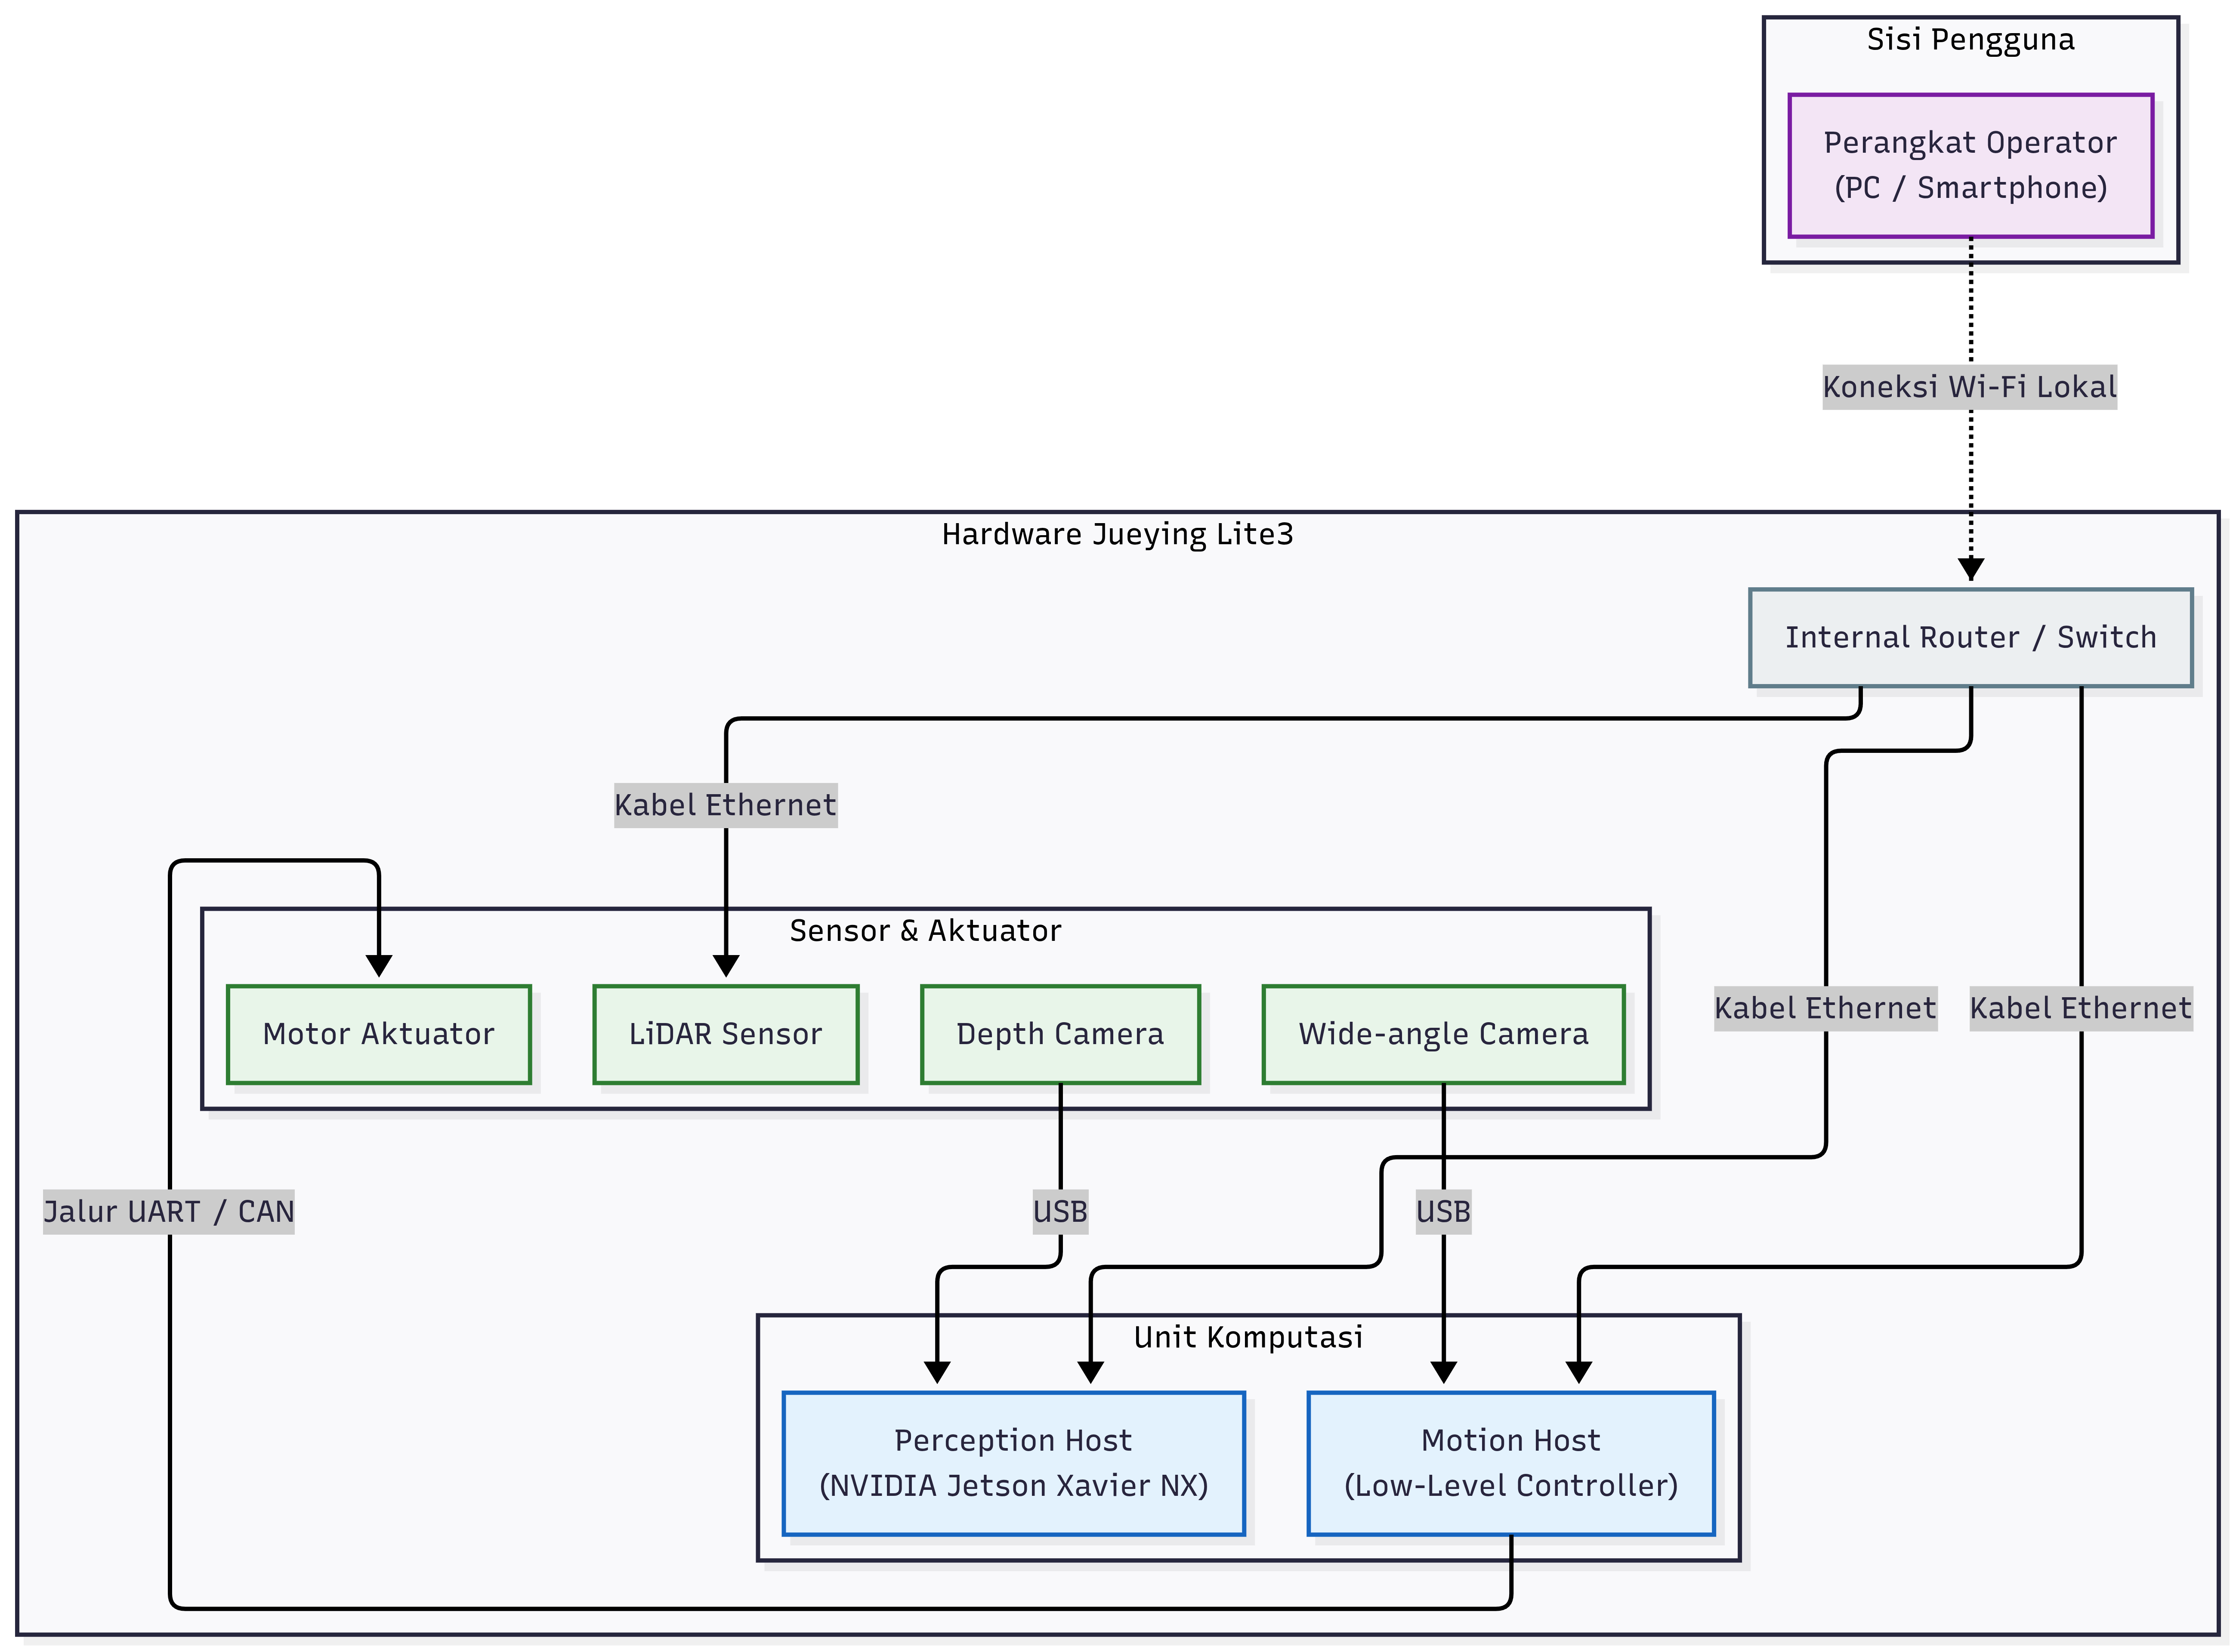
\includegraphics[width=0.8\textwidth]{Init/gambar/arsitektur_hardware.png}
%     \caption{Arsitektur Perangkat Keras Sistem Robot Inspeksi}
%     \label{fig:arsitektur_hardware}
% \footnotesize \textbf{Sumber:} Dokumentasi Penulis
% \end{figure}

\section{Implementasi Sistem}

\subsection{Penerapan Lokalisasi dan Pemetaan}

Proses pemetaan lingkungan dilakukan menggunakan algoritma Faster-LIO (\textit{LiDAR Inertial Odometry}) yang membangun peta awan titik 3D dalam format \textit{.pcd} dari data LiDAR dan IMU secara simultan. Prosedur pemetaan dimulai dengan menjalankan \textit{driver} LiDAR pada robot, diikuti dengan peluncuran \textit{node} Faster-LIO. Operator kemudian mengendalikan robot secara manual melalui aplikasi kendali untuk memindai seluruh area yang akan dipetakan. Setelah pemindaian selesai, program Faster-LIO dihentikan dan secara otomatis menyimpan file awan titik 3D ke direktori peta robot. File awan titik tersebut selanjutnya dikonversi menjadi peta grid 2D dalam format \textit{.pgm} menggunakan paket pcd\_2\_gridmap, yang menghasilkan peta okupansi yang dapat dibaca oleh \textit{Navigation Stack}.

Untuk proses lokalisasi, sistem menggunakan HDL Localization yang memanfaatkan algoritma NDT (\textit{Normal Distributions Transform}) dan Fast-GICP untuk mencocokkan data LiDAR \textit{real-time} dengan peta referensi. Algoritma ini menerima masukan berupa data awan titik dari sensor LiDAR dan peta referensi dalam format \textit{.pcd}, lalu menghasilkan estimasi pose robot (posisi dan orientasi) dalam \textit{frame} peta secara kontinu.

\begin{table}[H]
\centering
\caption{Komponen utama subsistem lokalisasi dan pemetaan}
\label{tab:slam-komponen}
\begin{tabular}{|l|l|l|}
\hline
\textbf{Proses} & \textbf{Algoritma/Paket} & \textbf{Output} \\ \hline
Pemetaan 3D & Faster-LIO & File awan titik (.pcd) \\ \hline
Konversi peta & pcd\_2\_gridmap & Peta grid 2D (.pgm) \\ \hline
Lokalisasi & HDL Localization (NDT + Fast-GICP) & Pose robot di frame map \\ \hline
\end{tabular}
\end{table}

\subsection{Penerapan Navigasi}

Navigasi otonom diimplementasikan menggunakan ROS \textit{Navigation Stack} dengan konfigurasi \textit{global planner} berbasis algoritma Dijkstra dan \textit{local planner} berbasis \textit{Timed Elastic Band} (TEB). Konfigurasi parameter utama navigasi ditunjukkan pada Tabel \ref{tab:nav-params}.

\begin{table}[H]
\centering
\caption{Parameter utama konfigurasi navigasi}
\label{tab:nav-params}
\begin{tabular}{|l|l|l|}
\hline
\textbf{Parameter} & \textbf{Nilai} & \textbf{Keterangan} \\ \hline
Global planner & Dijkstra & Jaminan jalur terpendek \\ \hline
Local planner & TEB & Perencanaan jalur elastis \\ \hline
max\_vel\_x & 0.5 m/s & Kecepatan linier maksimum \\ \hline
max\_vel\_theta & 1.0 rad/s & Kecepatan angular maksimum \\ \hline
min\_obstacle\_dist & 0.15 m & Jarak minimum ke rintangan \\ \hline
inflation\_dist & 0.3 m & Radius inflasi rintangan \\ \hline
\end{tabular}
\end{table}

Alur navigasi dimulai ketika MCP Server menerima pemanggilan \textit{tool} navigate\_to\_waypoint dari agen LLM. \textit{Controller} mengonversi koordinat tujuan menjadi \textit{MoveBaseGoal} dan mengirimkannya ke \textit{action server} move\_base. \textit{Global planner} menghitung jalur optimal di atas peta statis, kemudian \textit{local planner} TEB menerjemahkan jalur tersebut menjadi perintah kecepatan (cmd\_vel) yang dikirim secara berkala ke penggerak robot. Setelah robot mencapai tujuan atau gagal, \textit{callback} pada \textit{action client} mengirimkan laporan ke Backend melalui \textit{webhook}.

\subsection{MCP Server}

MCP Server merupakan komponen yang berjalan di sisi robot dan bertugas mengekspos kemampuan robot sebagai \textit{tools} yang dapat dipanggil oleh agen LLM. Server ini dibangun menggunakan pustaka FastMCP dan berjalan sebagai layanan HTTP pada port 8001. Saat dijalankan, server terlebih dahulu menginisialisasi \textit{node} ROS melalui ros\_manager yang membuat instansi \textit{Controller} dan menjalankan rospy.spin di \textit{thread} terpisah agar tidak memblokir server HTTP.

Tabel \ref{tab:mcp-tools} menunjukkan daftar lengkap \textit{tools} yang diekspos oleh MCP Server.

\begin{table}[H]
\centering
\caption{Daftar MCP Tools yang tersedia}
\label{tab:mcp-tools}
\begin{tabular}{|l|p{4cm}|p{3cm}|p{3cm}|}
\hline
\textbf{Tool} & \textbf{Fungsi} & \textbf{Input} & \textbf{Output} \\ \hline
move & Gerak manual (\textit{open-loop}) & kecepatan, durasi & Status \\ \hline
navigate\_to\_waypoint & Navigasi otonom via move\_base & x, y, theta & Status (async) \\ \hline
get\_object\_waypoints & Query objek inspeksi dari basis data & kata kunci, lokasi & Data waypoint \\ \hline
list\_sop\_files & Daftar file SOP & — & List filename \\ \hline
get\_sop\_file & Ambil file SOP & nama file & Info filepath \\ \hline
capture\_and\_upload\_image & Capture kamera, upload & — & URL gambar \\ \hline
\end{tabular}
\end{table}

Mekanisme pelaporan hasil aksi menggunakan pola \textit{webhook callback}. Setelah navigasi atau gerakan manual selesai, \textit{Controller} mengirimkan laporan berisi status keberhasilan dan detail aksi ke endpoint Backend melalui HTTP POST. Mekanisme ini memungkinkan agen LLM untuk menerima umpan balik dari robot dan melanjutkan rencana inspeksi secara kontekstual.

\subsection{Backend LLM Agent}

Backend LLM Agent merupakan layanan FastAPI yang berperan sebagai pusat koordinasi antara antarmuka web, agen LLM (Google Gemini), dan MCP Server. Layanan ini berjalan pada port 8082 dan menyediakan \textit{endpoint} /api/chat\_robot untuk menerima pesan dari \textit{dashboard} web maupun \textit{webhook callback} dari robot.

Inti dari Backend adalah mekanisme \textit{agentic loop} yang mengorkestrasi siklus percakapan antara Gemini dan MCP Server. Alur pemrosesan dimulai dengan pemuatan riwayat percakapan dari Supabase, dilanjutkan dengan pengiriman konteks ke Gemini API. Jika Gemini merespons dengan \textit{function\_call}, Backend meneruskan pemanggilan tersebut ke MCP Server, menerima hasilnya, dan menyuntikkan kembali ke konteks Gemini. Siklus ini berulang hingga Gemini menghasilkan respons teks final yang dikirimkan ke operator.

Proses injeksi file merupakan fitur penting dalam Backend. Ketika Gemini memanggil \textit{tool} get\_sop\_file atau capture\_and\_upload\_image, Backend tidak hanya meneruskan metadata hasil ke Gemini, tetapi juga mengunduh file asli dari Supabase Storage dan menyuntikkan \textit{bytes}-nya langsung ke konteks Gemini menggunakan Part.from\_bytes. Mekanisme ini memungkinkan Gemini untuk membaca isi dokumen SOP atau menganalisis gambar hasil \textit{capture} secara langsung. Saat memuat riwayat percakapan, proses injeksi ulang (\textit{re-injection}) file juga dilakukan agar konteks file tetap tersedia di sesi yang berlanjut.

Perilaku agen didefinisikan melalui \textit{system prompt} yang mengatur alur kerja inspeksi bertahap. \textit{Prompt} ini menginstruksikan Gemini untuk mengambil SOP terlebih dahulu, mencari koordinat objek, menyusun rencana inspeksi, meminta konfirmasi operator, mengeksekusi aksi satu per satu, menganalisis hasil gambar berdasarkan SOP, dan menanyakan kelanjutan kepada operator setelah setiap langkah.

\subsection{Antarmuka Web}

Antarmuka web dibangun menggunakan \textit{framework} Next.js dengan \textit{Tailwind CSS} sebagai aplikasi halaman tunggal yang terdiri dari delapan halaman. Komunikasi data menggunakan dua jalur, yaitu REST API ke Backend untuk operasi \textit{chat} dan manajemen data, serta \textit{WebSocket} melalui roslibjs ke rosbridge untuk menerima data telemetri \textit{real-time} dari ROS seperti posisi robot, peta okupansi, \textit{costmap}, dan \textit{video feed} kamera.

Tabel \ref{tab:web-pages} menunjukkan daftar halaman dan fungsinya.

\begin{table}[H]
\centering
\caption{Daftar halaman antarmuka web}
\label{tab:web-pages}
\begin{tabular}{|l|p{9cm}|}
\hline
\textbf{Halaman} & \textbf{Fungsi} \\ \hline
Inspection Hub & Halaman utama: peta navigasi + panel chat + video feed \\ \hline
SLAM Mapping & Memicu dan memantau proses pemetaan \\ \hline
Spatial Explorer & Manajemen hierarki lokasi (Map $\rightarrow$ Location $\rightarrow$ Waypoint) \\ \hline
Objects Manager & CRUD objek inspeksi beserta koordinat waypoint \\ \hline
SOP Documents & Pengunggahan dan pengelolaan dokumen SOP \\ \hline
Captured Gallery & Galeri gambar hasil capture kamera robot \\ \hline
Map Gallery & Galeri file peta yang tersimpan \\ \hline
Session History & Riwayat sesi percakapan dengan agen AI \\ \hline
\end{tabular}
\end{table}

% TODO: Tambahkan screenshot setiap halaman di sini
% Contoh:
% \begin{figure}[H]
% \centering
% \includegraphics[width=0.9\linewidth]{bab3/page_inspection_hub}
% \caption{Tampilan halaman Inspection Hub}
% \label{fig:page-inspection-hub}
% \end{figure}

\subsection{Basis Data dan Penyimpanan}

Sistem menggunakan Supabase sebagai layanan basis data yang dibangun di atas PostgreSQL. Skema basis data terdiri dari enam tabel utama yang saling berelasi untuk mendukung seluruh kebutuhan penyimpanan data sistem. Tabel \ref{tab:db-schema} menunjukkan struktur tabel yang digunakan.

\begin{table}[H]
\centering
\caption{Skema tabel basis data Supabase}
\label{tab:db-schema}
\begin{tabular}{|l|p{5cm}|p{5cm}|}
\hline
\textbf{Tabel} & \textbf{Kolom Utama} & \textbf{Relasi} \\ \hline
chat-sessions & id, title, created\_at & — \\ \hline
chat-messages & session\_id, role, content (JSON), showed & FK $\rightarrow$ chat-sessions \\ \hline
maps & id, name, metadata & — \\ \hline
locations & id, name, type, parent\_id, map\_id & FK $\rightarrow$ locations (self), FK $\rightarrow$ maps \\ \hline
objects & id, name, keywords[], sop\_url & — \\ \hline
object-waypoints & id, display\_name, view\_x/y/yaw, obj\_x/y, camera\_pan/tilt/zoom, parent\_id, object\_id & FK $\rightarrow$ locations, FK $\rightarrow$ objects \\ \hline
\end{tabular}
\end{table}

Selain basis data relasional, sistem juga memanfaatkan Supabase Storage untuk menyimpan file biner. Terdapat tiga folder utama dalam \textit{bucket} penyimpanan: folder sop/ untuk dokumen SOP dalam format PDF dan DOCX, folder captured/ untuk gambar hasil \textit{capture} kamera robot, dan folder maps/ untuk file peta dalam format \textit{.pgm}, \textit{.yaml}, dan \textit{.pcd}.

% TODO: Tambahkan diagram ER (TikZ) di sini
%\begin{figure}[H]
%\centering
%\caption{Diagram \textit{Entity-Relationship} basis data}
%\label{fig:er-diagram}
%\end{figure}

\subsection{Deployment dan Jaringan}

Seluruh komponen perangkat lunak di sisi robot dikelola menggunakan dua mekanisme. Empat \textit{service} utama dijalankan melalui \textit{systemd} agar dapat berjalan otomatis saat robot dinyalakan, yaitu lidar.service untuk \textit{driver} LiDAR, navigation.service untuk \textit{move\_base}, mcp-server.service untuk MCP Server pada port 8001, dan mcp-client.service untuk Backend FastAPI pada port 8082. Aplikasi \textit{dashboard} web dijalankan melalui Docker Compose pada port 3000.

Untuk konektivitas jarak jauh, robot dipasang Tailscale VPN yang memberikan alamat IP statis dalam jaringan \textit{mesh} privat. Dengan konfigurasi ini, operator tidak perlu berada dalam satu jaringan lokal dengan robot, melainkan cukup memiliki koneksi internet dan terdaftar dalam jaringan Tailscale yang sama. Layanan Supabase yang berjalan di komputer pengembang juga terhubung ke jaringan Tailscale yang sama, sehingga robot dapat mengakses basis data melalui \textit{tunnel} VPN tanpa memerlukan \textit{deployment} ke \textit{cloud} publik.

Tabel \ref{tab:services} menunjukkan daftar \textit{service} beserta konfigurasinya.

\begin{table}[H]
\centering
\caption{Daftar \textit{service} dan konfigurasi port}
\label{tab:services}
\begin{tabular}{|l|l|l|l|}
\hline
\textbf{Service} & \textbf{Port} & \textbf{Metode} & \textbf{Keterangan} \\ \hline
LiDAR driver & — & systemd & Publish topic /points\_raw \\ \hline
Navigation & — & systemd & move\_base + costmap \\ \hline
MCP Server & 8001 & systemd & FastMCP HTTP \\ \hline
Backend (MCP Client) & 8082 & systemd & FastAPI \\ \hline
Web Dashboard & 3000 & Docker Compose & Next.js \\ \hline
Rosbridge & 9090 & launch file & WebSocket bridge \\ \hline
Supabase & 54321 & laptop & PostgreSQL + REST \\ \hline
\end{tabular}
\end{table}

Urutan \textit{startup} sistem adalah sebagai berikut: pertama \textit{roscore} dijalankan, kemudian \textit{driver} LiDAR, navigasi (\textit{move\_base}), MCP Server, Backend (MCP Client), dan terakhir \textit{dashboard} web melalui docker-compose up.

% TODO: Tambahkan diagram deployment (TikZ) di sini
%\begin{figure}[H]
%\centering
%\caption{Diagram deployment sistem}
%\label{fig:deployment}
%\end{figure}
